\documentclass[12pt]{amsart}

\pagestyle{empty}

\usepackage{amsmath,amssymb,amsfonts,amsthm}
\usepackage{enumerate}% http://ctan.org/pkg/enumerate
\usepackage{eucal}

\usepackage{graphicx,psfrag} %only include if using pictures

\usepackage{ifthen} %only include if using conditional package

%\usepackage{xymatrix}


%keep this...%%%%%%%%%%%%%%%%%%%%%%%%%%%%%%%%%%%%%%%%%%%%%%%%%%%%
\vfuzz2pt % Don't report over-full v-boxes if over-edge is small
\hfuzz2pt % Don't report over-full h-boxes if over-edge is small
%%%%%%%%%%%%%%%%%%%%%%%%%%%%%%%%%%%%%%%%%%%%%%%%%%%%%%%%%%%%%%%%%

%Side Margins
\evensidemargin 0.1 in \oddsidemargin 0.1 in

%Paragraph Size
\parindent 24pt


%size of page
\textheight 9.6 in \textwidth 6.2 in
\baselineskip 9.6 in \topmargin 0.005 in


% ***********************************************************************
\newcommand{\Normalstretch}{1.0} %change to define space between lines
\renewcommand{\baselinestretch}{\Normalstretch}
\newenvironment{singlespace}
{\renewcommand{\baselinestretch}{1} \small \normalsize}
{\renewcommand{\baselinestretch}{\Normalstretch} \small \normalsize}
% ***********************************************************************
\newcommand{\baseenvskip}{\baselineskip 2mm}

% Standard Notation for Theorems and Lemmas
\newtheorem{mydef}{Definition}

\newtheorem{thm}{Theorem}

\newtheorem{lemma}[thm]{Lemma}

\newtheorem{claim}[thm]{Claim}

\newtheorem{proposition}[thm]{Proposition}

\newtheorem{conjecture}[thm]{Conjecture}

\newtheorem{corollary}[thm]{Corollary}

\theoremstyle{remark}
\newtheorem{rmk}{Remark}[section]
\newenvironment{remark}{\begin{rmk}\rm\baseenvskip}{\end{rmk}}
\newtheorem{definition}[rmk]{Definition}

%How numbering is defined in articles (standard)
\numberwithin{equation}{section} \numberwithin{thm}{section}
\numberwithin{rmk}{section} \numberwithin{figure}{section}

% ************************ space ************************************
\newcommand{\hhs}[1]{\hspace{#1mm}}
\newcommand{\hs}{\hspace{5mm}}
\newcommand{\vp}{\vspace{1mm}}
\newcommand{\vs}{\vspace{5mm}}
\newcommand{\jl}{$\frac{}{}$} %User defined for empty symbol to jump line
% ********************** newcommand *********************************
\newcommand{\mbf}[1]{\mbox{\boldmath $#1$}}
\newcommand{\hb}[1]{\hspace{-#1 mm}}
\newcommand{\ds}{\displaystyle}
\newcommand{\QED}{\hfill $\Box$}
% *********************** frequently used math symbols from AMS *******
\newcommand{\norm}[1]{\left\Vert#1\right\Vert}
\newcommand{\abs}[1]{\left\vert#1\right\vert}
\newcommand{\set}[1]{\left\{#1\right\}}

% ************** Some frequently used symbols - User defined ***********
% ************** Also Called MACROS ************************************

\newcommand{\N}{\mathbb{N}}
\newcommand{\Q}{\mathbb{Q}}
\newcommand{\Hv}{\mathcal{H}_v}
\newcommand{\h}{\mathcal{H}}
\newcommand{\Ov}{\mathcal{O}_v}
\newcommand{\F}{\mathcal{F}}
\newcommand{\Rn}{R^n}
\newcommand{\C}{\mathbb{C}}
\newcommand{\Ce}{\widehat{\mathbb{C}}}
\newcommand{\si}{\sigma}
\newcommand{\Cn}{\mathbb{C}^n}
\newcommand{\Z}{\mathbb{Z}}
\newcommand{\p}{\partial}
\newcommand{\ep}{\varepsilon}
\newcommand{\D}{\delta}
\newcommand{\eps}{\varepsilon}
\newcommand{\finv}{f^{-1}}
\newcommand{\im}{\imath}
\newcommand{\ga}{\gamma}
\newcommand{\ze}{\zeta}
\newcommand{\fee}{\varphi}
\newcommand{\noi}{\noindent}
%
% *******************************************************************
% At First run of Template, only modify from here below........ *****
% *******************************************************************


\begin{document}

\title{}

% ******************** ABSTRACT *************************************
%\begin{abstract}
%Insert abstract
%\end{abstract}
% Must be present so the above information is displayed.
% *******************************************************************
% **** Begin Typing your work from here below ***********************
% *******************************************************************


\textbf{
\section{{Q1.4 Conditional Probability}}
}

\vspace{2em}
Compute the conditional probability density of X, conditional on \( Y = y, \, f_{X \mid Y}(x \mid y) \). (Make sure you state the values of y for which this exists.)
\vspace{2em}

\begin{proof}

\begin{thm}[Theorem 1.1.8: Conditional Probability]
Let \( A, B \in S \) with \( P(B) > 0 \). Then the conditional probability of \( A \) given \( B \) is:
\[
P(A \mid B) = \frac{P(A \cap B)}{P(B)}
\]
\end{thm}
We can use this definition to translate the conditional PDF of X|Y to : Let A = x and y = B
\[
\frac{f_{X,Y}(x, y)}{f_Y(y)}
\]
then

\[
f_{X \mid Y}(x \mid y) = \frac{f_{X,Y}(x, y)}{f_Y(y)}
\]
1. Plug-in the joint PDF and marginal PDF from pervious questions:

joint PDF = $\frac{1}{2x}$ , 0<y<x<2
marginal = marginal = $\frac{1}{2} \ln\left( \frac{2}{y} \right)$


\[
f_{X \mid Y}(x \mid y) = \frac{\frac{1}{2x}}{\frac{1}{2} \ln\left( \frac{2}{y} \right)} = \frac{1}{x \ln\left( \frac{2}{y} \right)}
\]


We are given the conditional probability density function:
\[
f_{X \mid Y}(x \mid y) = \frac{1}{x \ln\left( \frac{2}{y} \right)}
\]

To compute its derivative with respect to \( x \), we first treat \( \ln\left( \frac{2}{y} \right) \) as a constant (since \( y \) is fixed) :(I verified the derivative using WolframAlpha

\[
f_{X \mid Y}(x \mid y) = \frac{1}{\ln\left( \frac{2}{y} \right)} \cdot \frac{1}{x}
\]

Multiple rule:
\[
\frac{d}{dx} f_{X \mid Y}(x \mid y) = \frac{1}{\ln\left( \frac{2}{y} \right)} \cdot \frac{d}{dx}\left( \frac{1}{x} \right)
\]

Differentiate \( \frac{1}{x} \) using the power rule:
\[
\frac{d}{dx}\left( \frac{1}{x} \right) = \frac{d}{dx}(x^{-1}) = -x^{-2} = -\frac{1}{x^2}
\]

Therefore, the derivative is:
\[
\frac{d}{dx} f_{X \mid Y}(x \mid y) = -\frac{1}{x^2 \ln\left( \frac{2}{y} \right)}
\]


\noindent
2. Define the support: From the joint PDF \( 0 < y < x < 2 \). When conditioning on \( Y = y \), this defines the range of \( x \) as:
\[
x \in (y, 2), \quad \text{for } y \in (0, 2)
\]

\noindent
Therefore, the full expression for the conditional PDF is:
\[
f_{X \mid Y}(x \mid y) =
\begin{cases}
\displaystyle \frac{1}{x \ln\left( \frac{2}{y} \right)}, & \text{if } y < x < 2 \text{ and } 0 < y < 2 \\
0 & \text{otherwise}
\end{cases}
\]




\vspace{1em}


\begin{figure}[h]
\centering
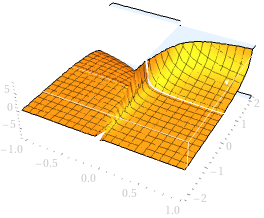
\includegraphics[width=0.6\textwidth]{conditionalpb-ruler.png}
\caption{3D surface plot of a function of \( x \) and \( y \). (e.g., conditional PDF \( f_{X \mid Y}(x \mid y) \))}
\label{fig:conditional_pdf}
\end{figure}




I computed the derivative using WolframAlpha\footnote{\url{https://www.wolframalpha.com}}.
\end{proof}

\end{document}